\begin{figure}[htbp]
\centering
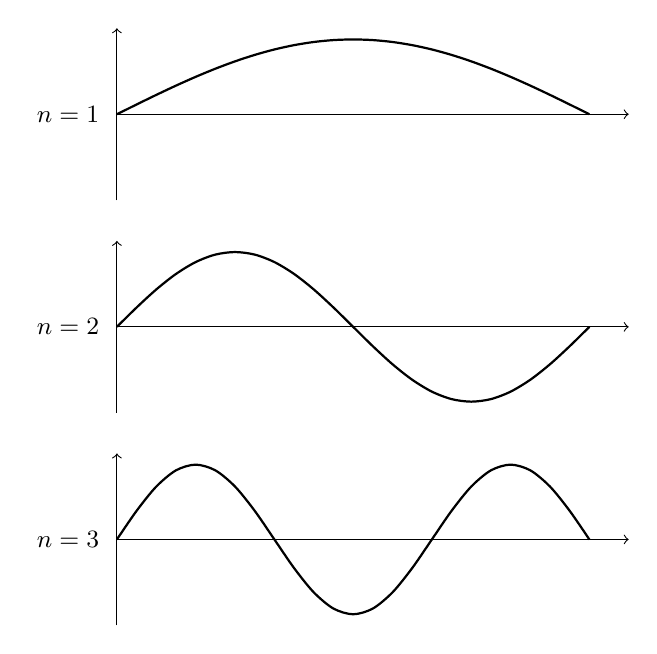
\begin{tikzpicture}[x=1cm,y=0.95cm]
\foreach \n/\yy in {1/0,2/-2.7,3/-5.4}{
  \begin{scope}[yshift=\yy cm]
  \draw[->] (0,0) -- (6.5,0);
  \draw[->] (0,-1.15) -- (0,1.15);
  \draw[thick,domain=0:360,smooth,variable=\t] plot ({\t/360*6}, {sin(\n*\t/2)});
  \node[left] at (-0.1,0) {\small $n=\n$};
  \end{scope}
}
\end{tikzpicture}
\caption{两端固定弦的前三个简正模。$n$ 是半波数，内部节点数为 $n-1$。}
\end{figure}
